\chapter{Indroduction}
The most popular information resource today is undoubtedly the internet. One of its key advantages is data availability. Frequently, data are stored on remote devices (commonly servers) and users can connect to these devices and access data they require. These data can contain private or secret information such as family pictures, passwords, bills or other sensitive content that need to be protected. Access to a server with this kind of sensitive information can be protected by some kind of authorization (for example login and password). But even the most secure kind of authorization is not sufficient enough to secure data from unauthorized access. For a user to obtain any type of content on a remote device, data must be transferred. In the case of the internet, data are transferred over multiple devices on which data can be accessed or even modified by a potential attacker (without the knowledge of either side of communication).

\begin{figure}[H]
    \begin{center}
        \label{img:unsecureConnection}
        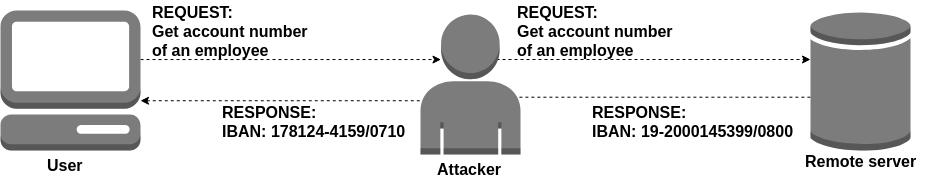
\includegraphics[width=1.0\textwidth]{obrazky-figures/unsecureconnection.png}
        \caption{Example of unauthorised data access and modification during its transmission.}
    \end{center}
\end{figure}

Usage of cryptography is the most frequently used solution for this problem. Data can be encrypted during the communication or encrypted data can be stored on servers and then transferred with or without further encryptions. This thesis will use the second approach, where data are already encrypted on a remote server. Under the term of data, you can imagine usual web page including not only text, images or videos but JavaScript and CSS as well. Some elements of this page (or even whole page) can be encrypted using an symmetric cypher and different parts can be encrypted using a different key or some parts can be encrypted using multiple keys. These keys are encrypted with asymmetric cypher and they are part of encrypted content as well. The outcome of this thesis will be a web browser extension that will be able to detect encrypted content (images, videos, text, etc.) and decrypt it for a user using his available keys. With this encryption/decryption system, users can create web pages where different data can be accessible for different users without the need for authentication on a remote server.

The target platform will be GNU/Linux and web extensions will be implemented for Firefox browser. Data will be decrypted with the Linux command line application called gpg, that will be used not only for decryption but for key management as well.

% \chapter{Theory}
% To develop functional and sufficient software for decrypting web pages, it is necessary to understand the tools we will work with. The purpose of this chapter is to introduce you to used technology in this thesis, such as GnuPG or WebExtensions. These tools have their advantages, disadvantages, and limits.

\chapter{The GNU Privacy Guard}
The GNU Privacy Guard, also known as GnuPG or GPG, is a complete and free implementation of the OpenPGP standard as defined by RFC4880 \cite{RFC4880}. GnuPG offers encryption, decryption and signing both data and communication. It features a versatile key management system with access modules for many kinds of public key directories. Not only that GnuPG is available for both Windows and Linux, but also a wealth of applications and libraries are available. \cite{GnuPG}

Linux implementation of GnuPG is a command line tool with features for integration with other applications. Windows version of GnuPG is Gpg4win with a context menu tool, a crypto manager, and an Outlook plugin to send and receive standard PGP/MIME mails. \cite{GnuPG}

\section{OpenPGP standard}
As mentioned earlier, GnuPG is the implementation of OpenPGP standard. Most of the text from this section is taken from RFC4880 \cite{RFC4880}. OpenPGP combines symmetric--key encryption and public--key encryption to provide confidentiality. First of all, the object is encrypted using a symmetric encryption algorithm. It is worth mentioning that each symmetric key is used only once for a single object. For each object, a new key is generated as a random number. This key is bound to the message and transmitted with it. Key is protected by encryption as well -- the key is encrypted with the receiver's public key. The sequence is as follows (also described in the figure \ref{img:messageEncryption}):
\begin{enumerate}
    \item A message is created by the sender.
    \item The sending OpenPGP generates a random number to be used as a session key for this message only.
    \item The generated session key is encrypted using recipient's public key. This encrypted session key starts the message.
    \item The sending OpenPGP encrypts the message using the session key, which forms the remainder of the message. Note that the message is also usually compressed.
    \item The receiving OpenPGP decrypts the session key using the recipient's private key.
    \item The receiving OpenPGP decrypts the message using the session key. If the message was compressed, it will be decompressed.
\end{enumerate}

\begin{figure}[H]
    \begin{center}
        \label{img:messageEncryption}
        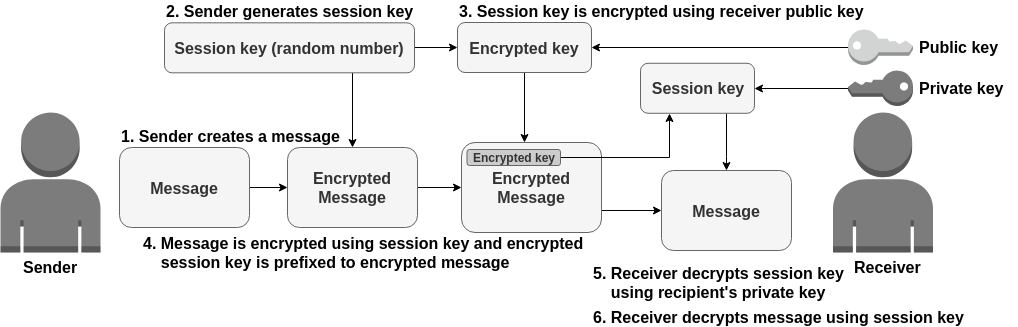
\includegraphics[width=1.0\textwidth]{obrazky-figures/messageEncryption.png}
        \caption{Schema of message encryption and decryption}
    \end{center}
\end{figure}

A symmetric key, that is used for message encryption, can be derived from a passphrase (or different kind of shared secret), or a two--stage mechanism similar to the public--key method that was described above in which a session key is itself encrypted with a symmetric algorithm keyed from a shared secret.

Authentication can be achieved using a digital signature. The digital signature uses a hash code or message digest algorithm, and a public--key signature algorithm. The sequence is as follows (also described in the figure \ref{img:messageSignature}):
\begin{enumerate}
    \item A message is created by the sender.
    \item The sending software generates a hash code of the message.
    \item The sending software generates a signature by encrypting hash code of message using the sender's private key.
    \item The binary signature is attached to the message.
    \item The receiving software keeps a copy of the message signature.
    \item The receiving software generates a new hash code for the received message and verifies it using the message's hash code obtained by decrypting signature with sender's private key.
\end{enumerate}

\begin{figure}[H]
    \begin{center}
        \label{img:messageSignature}
        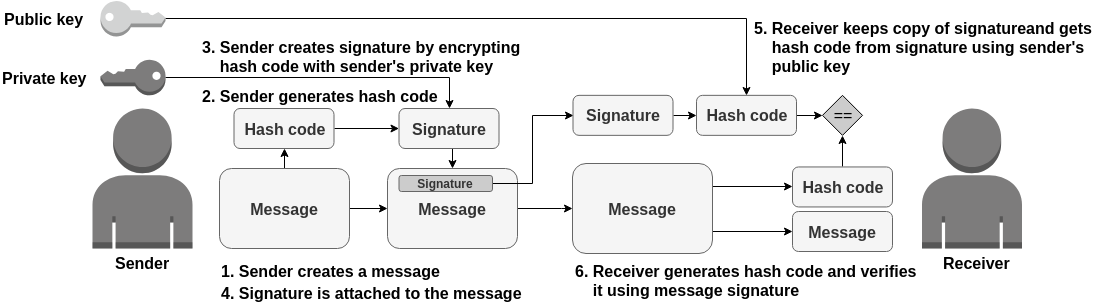
\includegraphics[width=1.0\textwidth]{obrazky-figures/messageSignature.png}
        \caption{Schema of message signature}
    \end{center}
\end{figure}

Both confidentiality and signature services may be applied to the same message. First signature is created and attached to the message. Then message (including signature) is encrypted using a symmetric session key. At last, this session key is encrypted with publickey encryption and prefixed to the encrypted message.

\section{GnuPG for Linux distributions}
As described above, there is a Linux application called gpg. It is important to have this application installed and configurated otherwise implemented software in this thesis will not work correctly or will not work at all. Reason for this is a fact, that GnuPG is not only used for decryption of encrypted elements but solves problems of the key management as well. Furthermore, the gpg application can be used for encryption of web pages as well.

Installation of GnuPG may differ on different operating systems. Some GNU/Linux distribution may already come with directly installable packages. However, it worth consider installation from the source code because the version of these packages may be old. The list of different GnuPG packages, libraries, required tools, optional software, legacy versions of GnuPG or manual can be found on GNU Privacy Guard web page \cite{GnuPG}.

\subsection{Basic Key Management}
Since objects are signed using the receiver's public key and decrypted with the receiver's private key, it is clear that receiver must have this keypair. Keypair is not only needed to encrypt messages but also to sign messages. With gpg installed on user's machine, the user can generate its own private and public keys. Basic key management will be further in these steps:
\begin{enumerate}
    \item Generating a new pair of private and public key
    \item Importing and exporting of both private and public keys
\end{enumerate}

\subsection*{Generating a New Pair of Private and Public Key}
To generate keypair with gpg, the user must complete several steps. The first step is to lunch gpg application with the argument \textit{--gen-key}. Next, the user is asked for a name and email address. From name and email address gpg creates a User ID. The User ID is something like a name tag for generated keypair and is also used to identify an owner of a public key.
\begin{Verbatim}[commandchars=\\\{\},codes={\catcode`$=3\catcode`_=8},samepage=true,frame=single]
xmatej52@merlin: ~\$ gpg --gen-key 
Real name: \textbf{Jiří Matějka}
E-mail address: \textbf{xmatej52@stud.fit.vutbr.cz}
You are using the 'utf-8' character set.
You selected this USER-ID:
    "Jiří Matějka <xmatej52@stud.fit.vutbr.cz>"

Change (N)ame, (E)mail, or (O)kay/(Q)uit?
\end{Verbatim}

Then the user is asked to enter a passphrase. The passphrase is used to encrypt private key so it is protected. If the passphrase is compromised, anyone who can access such private key will be able to decrypt owner's received messages or sign his messages as the owner of the private key. After the user enters the passphrase, gpg need to generate a lot of random bytes and ask the user to perform some other actions. After some time, keypair is finally generated.
\begin{Verbatim}[commandchars=\\\{\},codes={\catcode`$=3\catcode`_=8},samepage=true,frame=single]
\textbf{Enter passphrase:}
We need to generate a lot of random bytes. It is a good idea to perform
some other action (type on the keyboard, move the mouse, utilise the
disks) during the prime generation; this gives the random number
generator a better chance to gain enough entropy.

gpg: key 6C9359504F0C8F81 marked as ultimately trusted
gpg: revocation certificate stored as '/some/path/to/file'
public and secret key created and signed.

pub   rsa3072 2019-12-30 [SC] [expires: 2021-12-29]
      3252EA3A9A0F105E226BE7BF6C9359504F0C8F81
uid      Jiří Matějka <xmatej52@stud.fit.vutbr.cz>
sub   rsa3072 2019-12-30 [E] [expires: 2021-12-29]
\end{Verbatim}

\subsubsection*{Importing and Exporting of Both Private and Public Keys}


\subsection{Encrypting, Decrypting, Signing and Verifying Data}
\begin{enumerate}
    \item Encrypting files and text
    \item Decrypting files and text
    \item Signing data
    \item Verifying signed data
\end{enumerate}

\subsubsection*{Encrypting Files and Text}


\subsubsection*{Decrypting Files and Text}


\subsubsection*{Signing Data}


\subsubsection*{Verifing Signed Data}


\subsection*{Data Encyption and Decryption}


\subsection*{User Interface}
KGpg is KDE's application providing a simple interface for GnuPG. The application can help to set up and manage keys, import and export keys, view key signatures, trust status, expiry dates or encrypt/decrypt text or files. KGpg is a free and open source software, available for Linux and similar operating systems. Since KGpg provides user interface, KGpg makes it easy to work with the gpg command--line application so that user does not remember all the gpg's commands, particularly those for key management and data encryption/decryption. \cite{KGpg}

\section{Alternative software}
Although GnuPG is a very popular software and one of the most used implementations of OpenPGP standard implementation, there are some alternatives for GnuPGP that also implements OpenPGP standard. OpenPGP.js is one of such alternatives and was even used in this thesis for prototype development.

\subsection*{OpenPGP.js}
OpenPGP.js is a project that aims to provide an Open Source OpenPGP JavaScript library so it can be used on most of the devices. While many other implementations of OpenPGP standard are aimed at using native code, OpenPGP.js is meant to bypass this requirement so people are not forced to install gpg on their machines in order to use the library. The idea behind OpenPGP.js is to implement all the needed OpenPGP functionality in JavaScript library that can be reused in other projects that provides web browser extensions or server applications. \cite{OpenPGPjs}

OpenPGP.js library was used for the implementation of the first prototype \ref{prototype:OpenPGPjs}. Implemented prototype was able to encrypt and decrypt elements using hardcoded private and public keys in the source code. Accessing the user's public and private keys was a serious problem.  When background script and native application were developed, this library was no longer necessary and was replaced with gpg (using gpg also solved the problem with private and public key access).

\chapter{Browser Extensions}

\chapter{Draft and Implementation}

\section{OpenPGP.js Prototype}
\label{prototype:OpenPGPjs}


\chapter{Conclusion}
